% Runnable geometry example, not a domain algorithm or an experimental result.
% All stages and predicates below are synthetic. When adapting the figure,
% follow the actual source algorithm; do not invent a stage to fill a tier.
% This is an unscaled, full-size landscape figure. For a narrower publication
% frame, redesign or split the flow rather than shrinking its text and gaps.
% Compile with pdflatex; rasterize the resulting PDF at 300 dpi for visual QA.
\documentclass[tikz,border=12pt]{standalone}
\usepackage{amsmath}
\usetikzlibrary{arrows.meta,backgrounds,calc,positioning}

\definecolor{navy}{RGB}{30,48,70}
\definecolor{cardfill}{RGB}{247,249,251}
\definecolor{failure}{RGB}{120,57,42}

\begin{document}
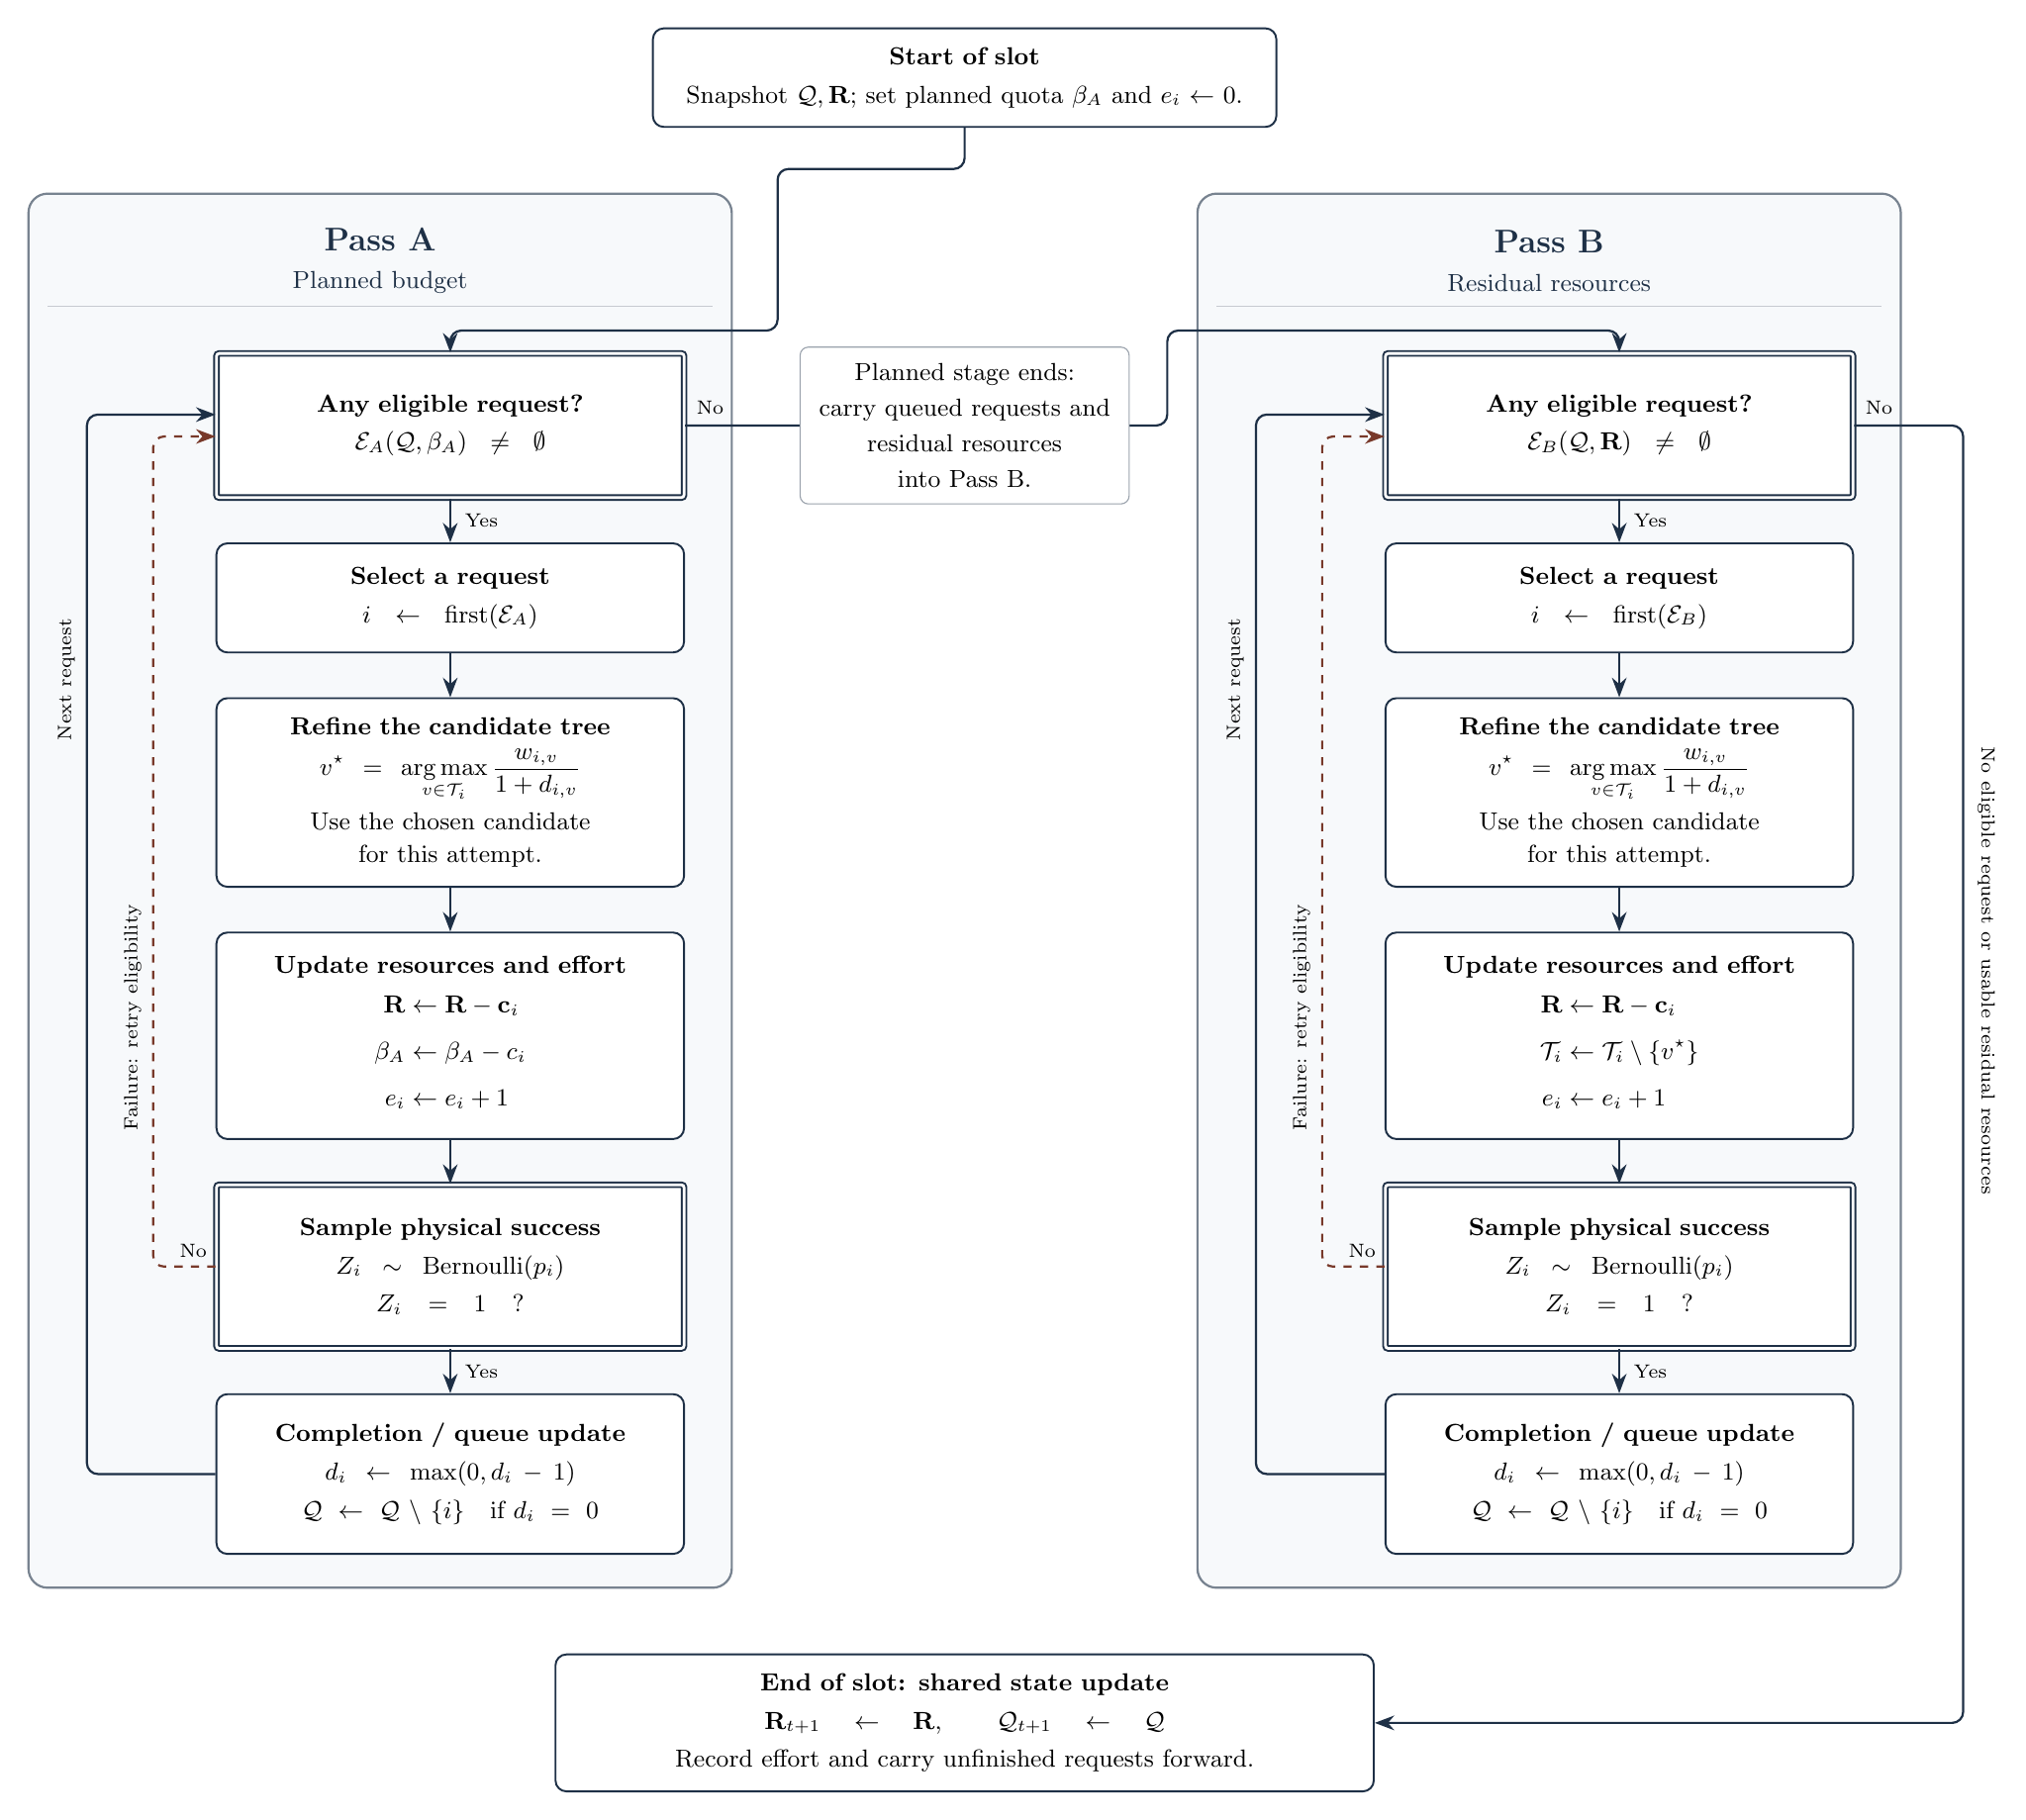
\begin{tikzpicture}[
  font=\small,
  block/.style={
    draw=navy, fill=white, line width=0.7pt, rounded corners=4pt,
    minimum width=6cm, text width=5.4cm, align=center, inner sep=7pt
  },
  decision/.style={
    block, rounded corners=1pt, double, double distance=1pt,
    minimum height=1.85cm
  },
  select/.style={block, minimum height=1.4cm},
  refine/.style={block, minimum height=2.2cm},
  update/.style={block, minimum height=2.65cm},
  sample/.style={decision, minimum height=2.1cm},
  complete/.style={block, minimum height=2.05cm},
  arr/.style={-{Stealth[length=2.5mm]}, draw=navy, line width=0.8pt},
  failarr/.style={arr, draw=failure, dashed},
  smalllabel/.style={font=\scriptsize, inner sep=1pt},
  returnlabel/.style={smalllabel, above=3pt, sloped},
  badge/.style={
    fill=white, draw=navy!45, rounded corners=3pt,
    text width=3.8cm, align=center, inner sep=6pt, font=\small
  },
  terminal/.style={block, minimum width=10.5cm, text width=10cm}
]

% Six matched functional tiers. Minimum heights cover the full rendered math;
% the positioning library measures the outer node edges before adding 16pt.
% Both columns use the same per-tier heights and unscaled font sizes.
\node[decision] (a-check) at (-6.5,0) {
  \textbf{Any eligible request?}\\[3pt]
  \(\mathcal E_A(\mathcal Q,\beta_A)\neq\emptyset\)
};
\node[decision] (b-check) at (8.5,0) {
  \textbf{Any eligible request?}\\[3pt]
  \(\mathcal E_B(\mathcal Q,\mathbf R)\neq\emptyset\)
};

\node[select, below=16pt of a-check] (a-select) {
  \textbf{Select a request}\\[3pt]
  \(i\leftarrow\operatorname{first}(\mathcal E_A)\)
};
\node[select] (b-select) at (b-check |- a-select) {
  \textbf{Select a request}\\[3pt]
  \(i\leftarrow\operatorname{first}(\mathcal E_B)\)
};

\node[refine, below=16pt of a-select] (a-refine) {
  \textbf{Refine the candidate tree}\\[4pt]
  \(\displaystyle
    v^\star=\operatorname*{arg\,max}_{v\in\mathcal T_i}
    \frac{w_{i,v}}{1+d_{i,v}}
  \)\\[3pt]
  Use the chosen candidate\\[1pt]
  for this attempt.
};
\node[refine] (b-refine) at (b-check |- a-refine) {
  \textbf{Refine the candidate tree}\\[4pt]
  \(\displaystyle
    v^\star=\operatorname*{arg\,max}_{v\in\mathcal T_i}
    \frac{w_{i,v}}{1+d_{i,v}}
  \)\\[3pt]
  Use the chosen candidate\\[1pt]
  for this attempt.
};

% Three explicit updates per pass. Pass A consumes its planned quota;
% this synthetic Pass B consumes a tree candidate instead. These differences
% illustrate geometry only and must be replaced by source-supported updates.
\node[update, below=16pt of a-refine] (a-update) {
  \textbf{Update resources and effort}\\[4pt]
  \(\begin{aligned}
    \mathbf R &\leftarrow \mathbf R-\mathbf c_i\\[3pt]
    \beta_A &\leftarrow \beta_A-c_i\\[3pt]
    e_i &\leftarrow e_i+1
  \end{aligned}\)
};
\node[update] (b-update) at (b-check |- a-update) {
  \textbf{Update resources and effort}\\[4pt]
  \(\begin{aligned}
    \mathbf R &\leftarrow \mathbf R-\mathbf c_i\\[3pt]
    \mathcal T_i &\leftarrow \mathcal T_i\setminus\{v^\star\}\\[3pt]
    e_i &\leftarrow e_i+1
  \end{aligned}\)
};

\node[sample, below=16pt of a-update] (a-sample) {
  \textbf{Sample physical success}\\[3pt]
  \(Z_i\sim\operatorname{Bernoulli}(p_i)\)\\[3pt]
  \(Z_i=1\;?\)
};
\node[sample] (b-sample) at (b-check |- a-sample) {
  \textbf{Sample physical success}\\[3pt]
  \(Z_i\sim\operatorname{Bernoulli}(p_i)\)\\[3pt]
  \(Z_i=1\;?\)
};

\node[complete, below=16pt of a-sample] (a-done) {
  \textbf{Completion / queue update}\\[3pt]
  \(d_i\leftarrow\max(0,d_i-1)\)\\[3pt]
  \(\mathcal Q\leftarrow\mathcal Q\setminus\{i\}\quad\text{if }d_i=0\)
};
\node[complete] (b-done) at (b-check |- a-done) {
  \textbf{Completion / queue update}\\[3pt]
  \(d_i\leftarrow\max(0,d_i-1)\)\\[3pt]
  \(\mathcal Q\leftarrow\mathcal Q\setminus\{i\}\quad\text{if }d_i=0\)
};

% Explicit card bounds are based on actual outer anchors, not text width.
% A 24mm left reserve contains both return lanes, their rotated label bounds,
% and border clearance. A 6mm right reserve contains the decision-port labels.
% The top includes a separate 58pt header band; the bottom is 12pt below the
% last node. The matched 9cm cards leave a 6cm inter-pass corridor.
\coordinate (a-left) at ([xshift=-24mm]a-check.west);
\coordinate (a-right) at ([xshift=6mm]a-check.east);
\coordinate (b-left) at ([xshift=-24mm]b-check.west);
\coordinate (b-right) at ([xshift=6mm]b-check.east);
\coordinate (card-top) at ([yshift=58pt]a-check.north);
\coordinate (card-bottom) at ([yshift=-12pt]a-done.south);
\coordinate (header-bottom) at ([yshift=17pt]a-check.north);
\coordinate (header-center) at ([yshift=33.5pt]a-check.north);
\coordinate (entry-level) at ([yshift=8pt]a-check.north);

\begin{scope}[on background layer]
  \draw[draw=navy!60, fill=cardfill, line width=0.8pt, rounded corners=7pt]
    (a-left |- card-top) rectangle (a-right |- card-bottom);
  \draw[draw=navy!60, fill=cardfill, line width=0.8pt, rounded corners=7pt]
    (b-left |- card-top) rectangle (b-right |- card-bottom);
\end{scope}

\node[align=center, text=navy] (a-header)
  at ($ (a-left |- header-center)!0.5!(a-right |- header-center) $) {
    \large\bfseries Pass A\\[3pt]\small Planned budget
  };
\node[align=center, text=navy] (b-header)
  at ($ (b-left |- header-center)!0.5!(b-right |- header-center) $) {
    \large\bfseries Pass B\\[3pt]\small Residual resources
  };
\draw[navy!25] ([xshift=7pt]a-left |- header-bottom)
  -- ([xshift=-7pt]a-right |- header-bottom);
\draw[navy!25] ([xshift=7pt]b-left |- header-bottom)
  -- ([xshift=-7pt]b-right |- header-bottom);

% Initialization uses the east-side corridor below the title band, then enters
% the eligibility node through its north port.
% The slot-start wire and the later A-to-B transfer occupy distinct corridors.
\node[block, minimum width=8cm, text width=7.4cm, anchor=south]
  (start) at ([yshift=24pt]0.1,0 |- card-top) {
    \textbf{Start of slot}\\[3pt]
    Snapshot \(\mathcal Q,\mathbf R\); set planned quota \(\beta_A\) and \(e_i\leftarrow0\).
  };
\coordinate (start-turn) at ([yshift=9pt]0.1,0 |- card-top);
\draw[arr, rounded corners=4pt] (start.south) -- (start-turn)
  -- (-2.3,0 |- start-turn) -- (-2.3,0 |- entry-level)
  -- (a-check |- entry-level) -- (a-check.north);

\foreach \p in {a,b} {
  \draw[arr] (\p-check.south) --
    node[smalllabel, right=4pt] {Yes} (\p-select.north);
  \draw[arr] (\p-select.south) -- (\p-refine.north);
  \draw[arr] (\p-refine.south) -- (\p-update.north);
  \draw[arr] (\p-update.south) -- (\p-sample.north);
  \draw[arr] (\p-sample.south) --
    node[smalllabel, right=4pt] {Yes} (\p-done.north);

  % Distinct west ports, two internal vertical lanes, and staggered labels.
  % Positions apply only to each vertical segment. Their label centers are
  % separated by more than 3cm; dashed failure also survives grayscale.
  \coordinate (\p-fail-lane) at ([xshift=-8mm]\p-check.west);
  \coordinate (\p-next-lane) at ([xshift=-16.5mm]\p-check.west);
  \coordinate (\p-fail-port) at ([yshift=-4pt]\p-check.west);
  \coordinate (\p-next-port) at ([yshift=4pt]\p-check.west);
  \draw[failarr, rounded corners=4pt]
    (\p-sample.west) -- (\p-fail-lane |- \p-sample)
    -- node[returnlabel, pos=0.30] (\p-fail-label) {Failure: retry eligibility}
       (\p-fail-lane |- \p-fail-port) -- (\p-fail-port);
  \node[smalllabel, anchor=south east, xshift=-2pt, yshift=2pt]
    at (\p-sample.west) {No};
  \draw[arr, rounded corners=4pt]
    (\p-done.west) -- (\p-next-lane |- \p-done)
    -- node[returnlabel, pos=0.75] (\p-next-label) {Next request}
       (\p-next-lane |- \p-next-port) -- (\p-next-port);
}

% A long transfer badge sits on a straight segment in the 6cm corridor.
% The bend is beyond the badge, so visible stem remains on both sides.
% Pass B enters from the north below its header, above both return lanes.
\draw[arr, rounded corners=4pt] (a-check.east)
  -- (2.7,0) -- (2.7,0 |- entry-level)
  -- (b-check |- entry-level) -- (b-check.north);
\node[smalllabel, anchor=south west, xshift=3pt, yshift=3pt]
  at (a-check.east) {No};
\node[badge] (transfer-label) at (0.1,0) {
  Planned stage ends:\\[2pt]
  carry queued requests and\\[2pt]
  residual resources\\[2pt]
  into Pass B.
};

% Shared termination is centered below the matched card pair. Its north edge
% clears the card bottom by 24pt (more than the required 20pt).
\coordinate (end-level) at ([yshift=-24pt]card-bottom);
\node[terminal, anchor=north] (end) at (0.1,0 |- end-level) {
  \textbf{End of slot: shared state update}\\[3pt]
  \(\mathbf R_{t+1}\leftarrow\mathbf R,\qquad
    \mathcal Q_{t+1}\leftarrow\mathcal Q\)\\[3pt]
  Record effort and carry unfinished requests forward.
};

% The global exit lane is 8mm beyond the right border. Its long explanation
% is sloped along the outer vertical segment, keeping the canvas compact.
\coordinate (exit-lane) at ([xshift=8mm]b-right);
\draw[arr, rounded corners=4pt] (b-check.east)
  -- (exit-lane |- b-check)
  -- node[smalllabel, above=4pt, sloped, pos=0.42] (exit-label)
       {No eligible request or usable residual resources}
     (exit-lane |- end.east)
  -- (end.east);
\node[smalllabel, anchor=south west, xshift=3pt, yshift=3pt]
  at (b-check.east) {No};

\end{tikzpicture}
\end{document}
